\documentclass[10pt]{beamer}

\usetheme[progressbar=frametitle]{metropolis}
\usepackage{appendixnumberbeamer}
\usepackage{lipsum}
\usepackage{amsmath}
\usepackage{amssymb}
\usepackage{booktabs}
\usepackage[scale=2]{ccicons}
\usepackage{pgfplots}
\usepgfplotslibrary{dateplot}
\usepackage{dirtytalk}
\usepackage{xspace}
\newcommand{\themename}{\textbf{\textsc{metropolis}}\xspace}
\definecolor{mpigreen}{HTML}{007977}
\setbeamercolor{frametitle}{bg=mpigreen}
%https://www.overleaf.com/project/60692a72c2db80145723d37f
\title{Microsoft Bot Framework}

\author{Tai Ng (ML Engineer)}

\institute{VINBRAIN INTERNSHIP PROGRAM 2021 }
\titlegraphic{\hfill
\includegraphics[height=3cm]{logo.png}}

\begin{document}


\maketitle

\begin{frame}{Introduction}
    \begin{figure}[H]
	\centering
	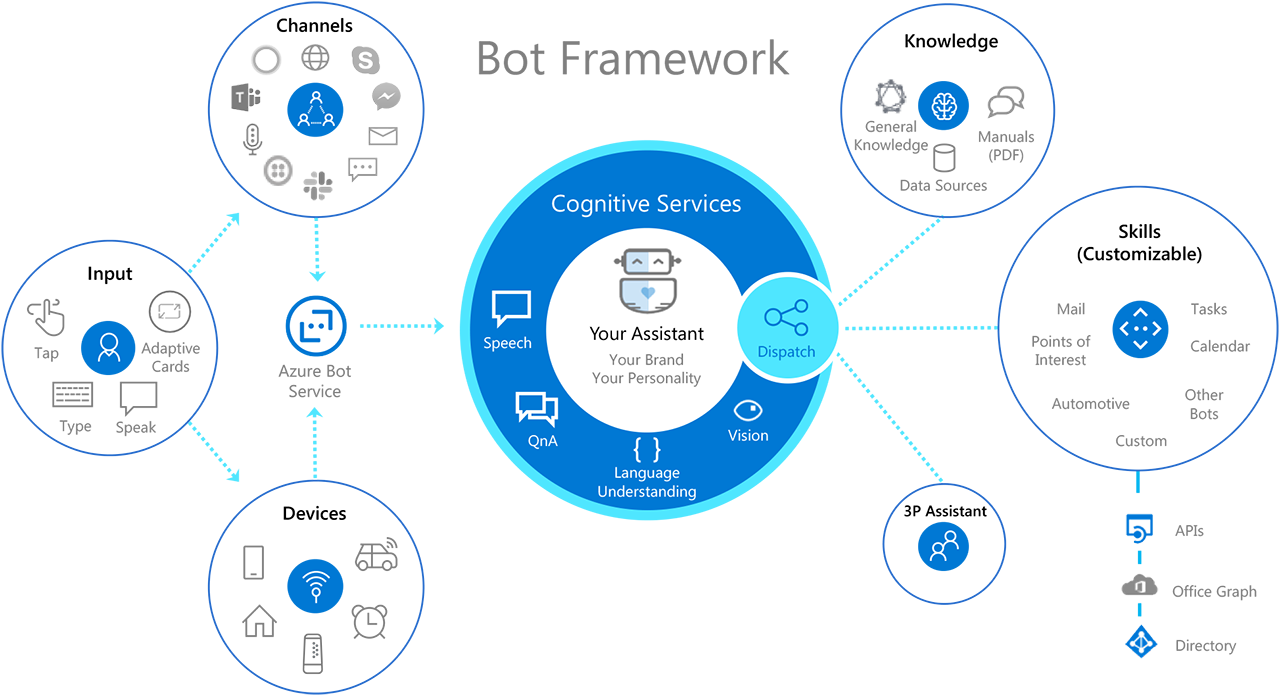
\includegraphics[width=10cm]{image/BotFrameworkDiagram.png}\par
	\caption{Components of a conversational AI experience}
	\label{fig:intro_bot}
    \end{figure}
\end{frame}

\begin{frame}{Building a Bot}
    \begin{figure}[H]
	\centering
	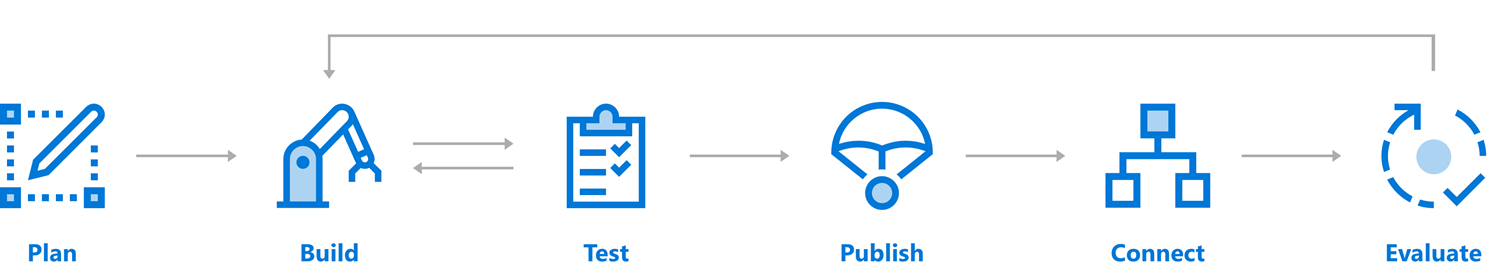
\includegraphics[width=10cm]{image/bot-service-overview.png}\par
	\caption{Pipeline}
	\label{fig:pipeline}
    \end{figure}
\end{frame}

\begin{frame}{User's Input}
	
\end{frame}

\begin{frame}{Conclusion}
    \begin{center}
        Q\&A
    \end{center}
\end{frame}

\end{document}
